% !TEX root =  main.tex

\chapter{Database design}\label{ch:db_design}



The database resides in a PostgreSQL DBMS.

\section{Schema: core}
The central part of the database schema is shown in figure \ref{figureDbCoreModel} and explained below:

\begin{figure}[H]
    \centering
    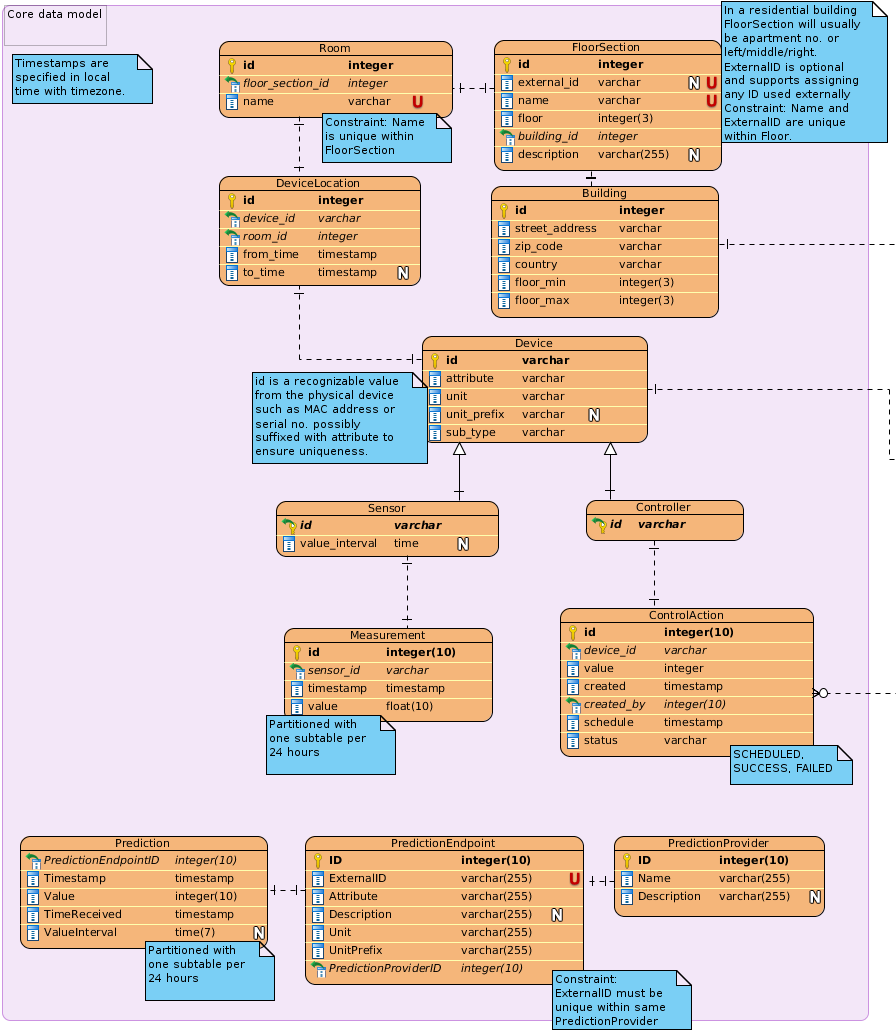
\includegraphics[width=\textwidth]{figures/db_core_schema}
    \caption{Database core schema}
    \label{figureDbCoreModel}
\end{figure}

\subsubsection{Devices and measurements}

\paragraph{Device} 
Entries in \texttt{Device} correspond to physical control and sensor devices, with the modification that we store one logical device for each function of the physical device. Whether a device is a sensor or a controller is specified by its presence in table \texttt{Controller} or \texttt{Sensor}. Columns \texttt{Attribute}, \texttt{Unit} and \texttt{UnitPrefix} (such as milli) are for sensors specification of the incoming measurement values, while they for controllers specify the format of values to send to the controller when actuating it.

\paragraph{Sensor} 
Table \texttt{Sensor} specifies an optional property \texttt{ValueInterval} which is used when measurement values are aggregated over a limited time interval (such as 15 minutes). 

\paragraph{Measurement} 
This table will contain a row for each measurement received from a physical sensor. It will simply consist of a \texttt{Value}, a \texttt{Timestamp} and a reference into \texttt{Sensor}, which enables interpretation of the value. The \texttt{Measurement} table is expected to grow very large and will therefore be partitioned into subtables that will each contain 24 hours of measurements and can be discarded on the fly according to the rolling window strategy explained in section \ref{subsection:rollingwindow}.

\paragraph{ControlAction} 
Table \texttt{ControlAction} will contain scheduled and past commands for controllers. An action is simply specified by a \texttt{Value} which can be interpreted via the reference into table \texttt{Controller} and \texttt{Device}. Column \texttt{Schedule} specifies the time for carrying out the action, and \texttt{Status} indicates if execution is still pending or has been completed. Finally, \texttt{IssuedBy} specifies which user scheduled the action. We might consider partitioning and discarding of old data in this table in the same way as for table \texttt{Measurement}.

\paragraph{Building, FloorSection, Room}
The physical properties of a building are modeled in these tables. A building consists of an integer range of floors. Each floor consists of \texttt{FloorSection}s which in most cases will be equivalent to apartments. The generalized term FloorSection is intended to support other types of buildings where designations such as "South wing" or other may be desired. Finally, a floor consists of named \texttt{Room}s. We do not expect to obtain device locations with a higher degree of accuracy than individual rooms.

\paragraph{DeviceLocation} This table maps \texttt{Device}s to \texttt{Room}s for specified time periods, indicating that devices may be moved around.

\subsubsection{Predictions}
Predictions of a wide range of values (power consumption, grid load, price, CO\textsubscript{2} emissions, ...) will be received from external data providers and will in addition be generated by our own application logic. 

While the data stored for predictions is quite similar to those for measurements, we have chosen to store them separately because of the fundamentally different semantics.

\paragraph{PredictionProvider}
An entity providing predictions, such as energinet.dk or the system itself.

\paragraph{PredictionEndpoint} 
A logical source of predictions of one type. Specifies the \texttt{Attribute}, \texttt{Unit} and \texttt{UnitPrefix} of the incoming values and provides an optional \texttt{Description}.

\paragraph{Prediction}
Actual prediction values. \texttt{Timestamp} indicates the time for which the value applies, while \texttt{TimeReceived} indicates when the prediction was received from the provider. This is relevant since multiple predictions for the same future point in time may be received over time. Some values actually cover an interval (for instance predicted power consumption for a given day of 24 hours), which is specified in column \texttt{ValueInterval}.
This table is also expected to grow quickly, motivating the same partitioning and rolling window strategy as for table \texttt{Measurement}.

\newpage


\subsection{Rolling window}\label{subsection:rollingwindow}
Since the \texttt{Measurement} table will grow very quickly, a partitioning and data discarding scheme will be employed. The table will be partitioned in time intervald, having one subtable for every 24 hours. Furthermore, subtables older than one week will be dropped. The time limits can naturally be configured. The same scheme might be applied to tables \texttt{ControlAction} and \texttt{Prediction}.
This is done in order to accommodate the VPP server on a desktop size machine with limited disk space.

\subsection{Data warehouse}
In order to retain data, the VPP will periodically forward data to an external database (data warehouse) that can accommodate a larger volume of data for longer periods. When forwarding data, measurements may be averaged over limited time intervals to reduce data size. The data warehouse can then be used for statistics and historical analysis. While the data warehouse schema was initially planned to be identical to the VPP rolling window DB, the presence of users, privileges and most likely various other configuration indicates that probably only the core schema as shown in figure \ref{figureDbCoreModel} should be present in the data warehouse. 

\subsection{CIM compliance}
The Common Information Model (CIM) is being taken into consideration in the design. Where it is applicable, we will aim to make our data model compliant. Units, unit prefixes, timestamps and time durations will be formatted to agree with CIM. On the other hand, CIM does not provide any guidance on how to structure for instance the building/floor/room model.

